%%%%%%%%%%%%%%%%%%%%%%%%%%%%%%%%%%%%%%%%%
% Beamer Presentation
% LaTeX Template
% Version 1.0 (10/11/12)
%
% This template has been downloaded from:
% http://www.LaTeXTemplates.com
%
% License:
% CC BY-NC-SA 3.0 (http://creativecommons.org/licenses/by-nc-sa/3.0/)
%
%%%%%%%%%%%%%%%%%%%%%%%%%%%%%%%%%%%%%%%%%

%-------------------------------------------------------------------------------
%	PACKAGES AND THEMES
%-------------------------------------------------------------------------------

\documentclass{beamer}
\usepackage{xcolor}
\usepackage{graphicx}
\usepackage{tikz}
\usepackage{listings}
\usepackage{multicol}

\DeclareMathOperator{\diag}{diag}

\definecolor{applegreen}{rgb}{0.55, 0.71, 0.0}
\definecolor{blue(ncs)}{rgb}{0.0, 0.45, 0.60}
\definecolor{burgundy}{rgb}{0.5, 0.0, 0.13}

\definecolor{cadet}{rgb}{0.33, 0.41, 0.47}
\definecolor{airforceblue}{rgb}{0.36, 0.54, 0.66}

\mode<presentation> {

\usetheme{CambridgeUS}

\usecolortheme{wolverine}

\definecolor{gold}{HTML}{D4A017}
\definecolor{darkgold}{HTML}{B7950B}

\setbeamercolor{palette primary}{bg=cadet,fg=white}
\setbeamercolor{palette secondary}{bg=airforceblue,fg=white}
\setbeamercolor{palette tertiary}{bg=black,fg=white}
\setbeamercolor{palette quaternary}{bg=cadet,fg=white}

\setbeamercolor{frametitle}{bg=airforceblue,fg=white}

\setbeamercolor{section number projected}{bg=black,fg=cadet}
\setbeamercolor{item}{fg=black,bg=cadet}

\setbeamertemplate{page number in head/foot}[framenumber]

\lstset{basicstyle=\ttfamily\footnotesize,breaklines=true}
}



\lstdefinestyle{colouredC}{ 
  commentstyle=\color[gray]{0.4},
  keywordstyle=\bfseries,
  keywordstyle=[2]\color[rgb]{0.75, 0, 0},
  keywordstyle=[3]\color[rgb]{0, 0.5, 0},
  keywordstyle=[4]\color[rgb]{0, 0.5, 0},
  keywordstyle=[5]\color[rgb]{0, 0, 0.75},
  numberstyle=\tiny\color{mGray},
  stringstyle=\color[rgb]{0, 0, 0.5},
  basicstyle=\ttfamily,
  language=C,
  morekeywords=[3]{CeedInt, CeedScalar},
}

\lstdefinestyle{boxedC}{
  style=colouredC,
  numbers=left,
  firstnumber=auto,
  numberblanklines=true,
  frame=trbL,
  numberstyle=\tiny,
  frame=leftline,
  numbersep=7pt,
  framesep=5pt,
  framerule=10pt,
  xleftmargin=15pt,
  backgroundcolor=\color[gray]{0.97},
  rulecolor=\color[gray]{0.90}%
}

\usepackage{graphicx} % Allows including images
\usepackage{booktabs} % Allows the use of \toprule, \midrule and \bottomrule in tables

%----------------------------------------------------------------------------------------
%	TITLE PAGE
%----------------------------------------------------------------------------------------

\title[libCEED]{PETSc with libCEED - Performance Portable Matrix-Free Operators
} % The short title appears at the bottom of every slide, the full title is only on the title page

\author{Jeremy L Thompson} % Your name
\institute[CU Boulder] % Your institution as it will appear on the bottom of every slide, may be shorthand to save space
{University of Colorado Boulder \\ % Your institution for the title page
\medskip
\textit{jeremy@jeremylt.org} % Your email address
}
\date{24 May 2024} % Date, can be changed to a custom date

\begin{document}

\begin{frame}
\titlepage % Print the title page as the first slide
\end{frame}

%------------------------------------------------

\begin{frame}
\frametitle{libCEED Examples Team}

\begin{center}
\includegraphics[height=2.75cm]{libCEEDlogo.png}
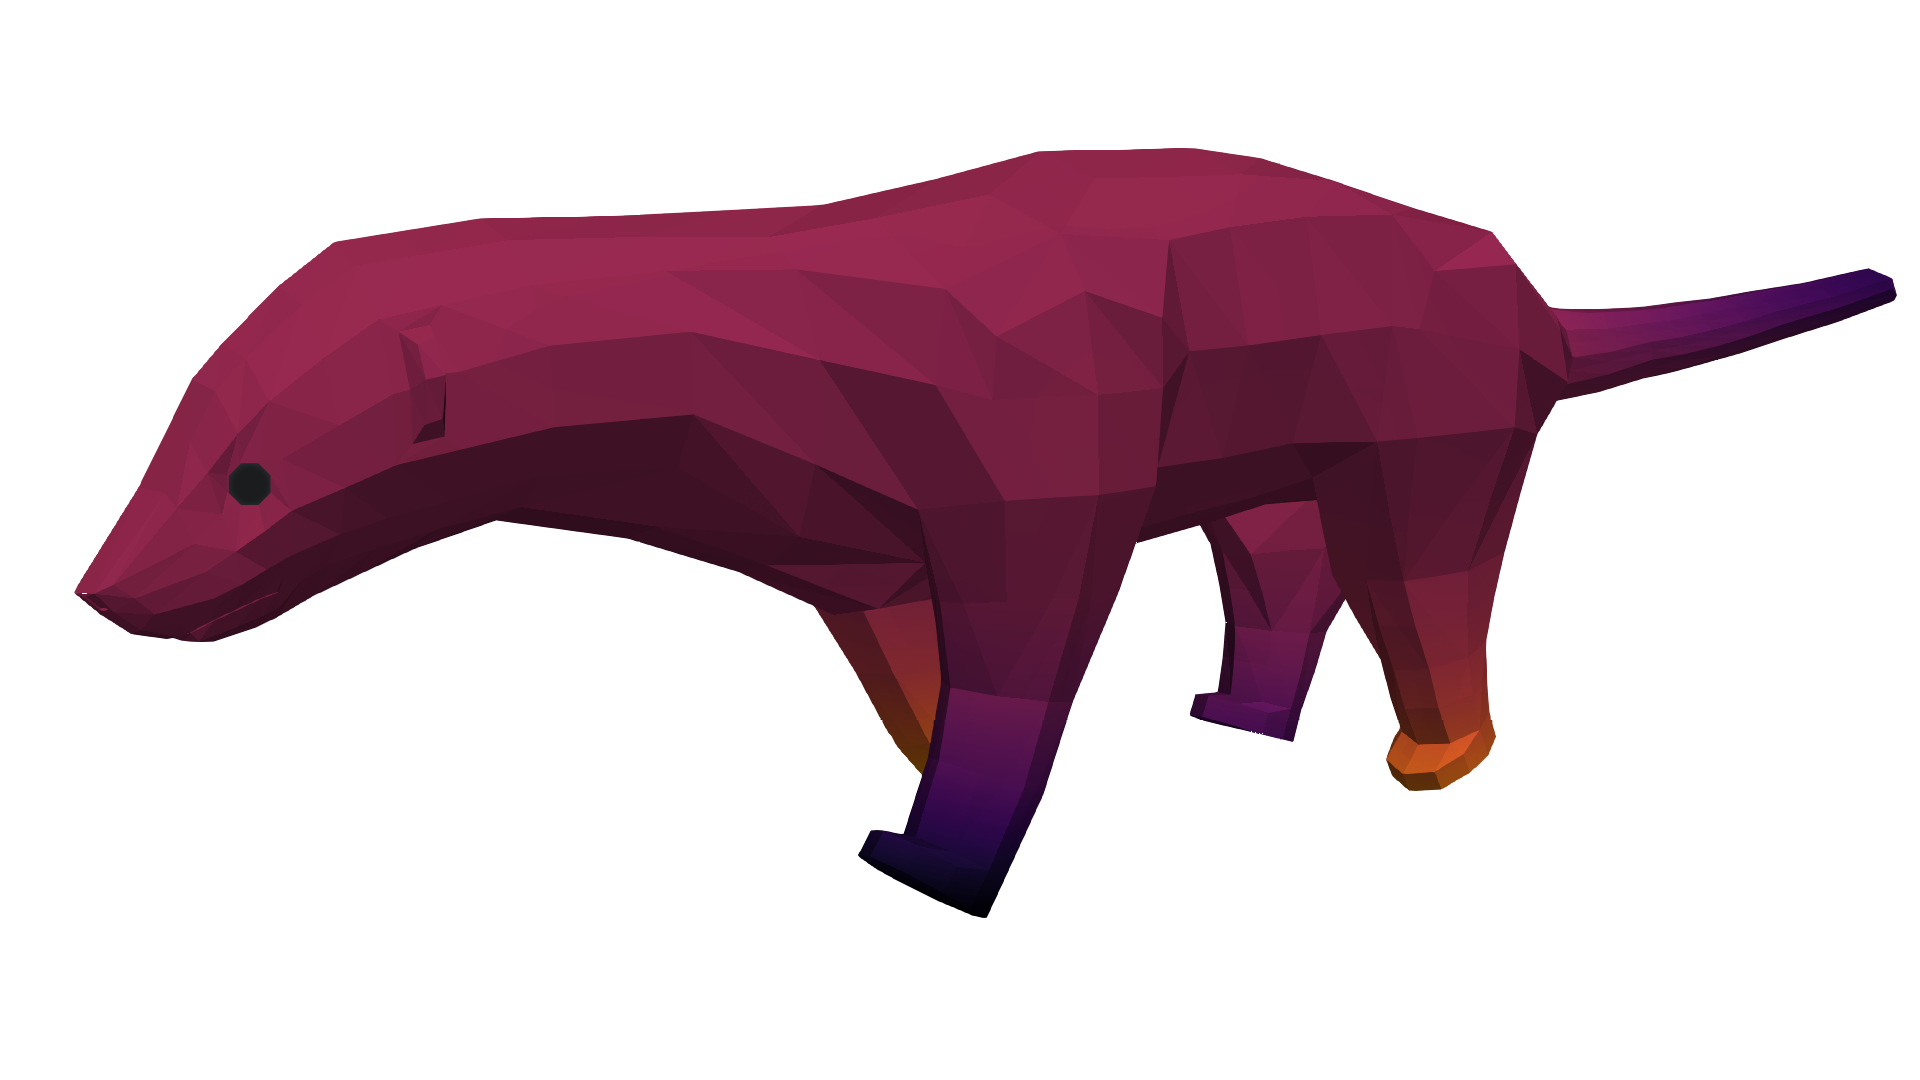
\includegraphics[height=2.75cm]{Ratellogo.png}
\end{center}

{\flushleft

libCEED Repo: https://github.com/CEED/libCEED\\
Ratel Repo: https://gitlab.com/micromorph/ratel\\

~\\
Developers: Zach Atkins, Jed Brown, Leila Ghaffari, Kenneth Jansen\\
\hspace{19mm} Rezgar Shakeri, James Wright, Jeremy L Thompson\\

~\\

{\tiny The authors acknowledge support by the Department of Energy, National Nuclear Security Administration, Predictive Science Academic Alliance Program (PSAAP) under Award Number DE-NA0003962.}

}

\begin{center}

\includegraphics[height=0.7cm]{psaap-center-logos}
\end{center}

\end{frame}

%------------------------------------------------

\begin{frame}
\frametitle{Overview} % Table of contents slide, comment this block out to remove it
\tableofcontents % Throughout your presentation, if you choose to use \section{} and \subsection{} commands, these will automatically be printed on this slide as an overview of your presentation
\end{frame}

%------------------------------------------------
\section{Background}
%------------------------------------------------

\begin{frame}
\begin{center}
\frametitle{ECP Roots}

\begin{itemize}

\item libCEED + PETSc projects follow from ECP CEED work\\

~\\

\item libCEED provides high-performance operator evaluation\\

~\\

\item libCEED provides CUDA, ROCm, and SYCL support\\

~\\

\item PETSc provides linear/non-linear solvers and time steppers\\

\end{itemize}

\end{center}
\end{frame}

%-------------------------------------------------------------------------------

\begin{frame}
\begin{center}
\frametitle{libCEED Projects}

Several projects built using libCEED\\

~\\

\begin{itemize}

\item Ratel - solid mechanics FEM and MPM (PSAAP)\\

~\\

\item HONEE - fluid dynamics FEM \& differential filtering (PHASTA)\\

~\\

\item MFEM - various applications, libCEED integrators (LLNL)\\

~\\

\item Palace - Electromagnetics FEM with MFEM + libCEED (Amazon)\\

~\\

\item RDycore - River dynamical core with PETSc + libCEED (SciDAC)\\

\end{itemize}

\end{center}
\end{frame}

%------------------------------------------------

\begin{frame}
\begin{center}
\frametitle{Matrix-Free Operators from libCEED}

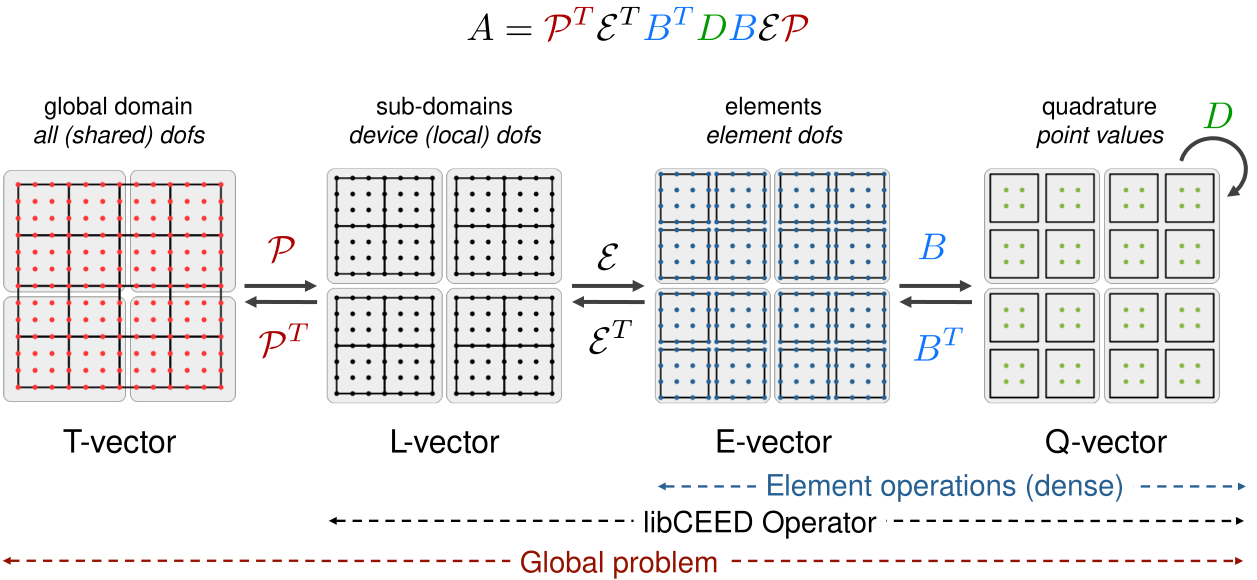
\includegraphics[height=5.0cm]{libCEEDAPI.png}

~\\

libCEED provides arbitrary order matrix-free operator evaluation\\

\end{center}
\end{frame}

%------------------------------------------------

\begin{frame}[fragile]
\begin{center}
\frametitle{Neo Hookean QFunction}

{\tiny
\begin{lstlisting}[style=boxedC]
static int ElasticityResidual_NeoHookean(void *ctx, CeedInt Q,
                               const CeedScalar *const *in, CeedScalar *const *out) {
  // Inputs
  const CeedScalar(*q_data)[CEED_Q_VLA] = (const CeedScalar(*)[CEED_Q_VLA])in[0];
  const CeedScalar(*ug)[CEED_Q_VLA][Q]  = (const CeedScalar(*)[3][CEED_Q_VLA])in[1];

  // Outputs
  CeedScalar(*grad_u)[3][CEED_Q_VLA] = (CeedScalar(*)[3][CEED_Q_VLA])out[0];

  // Context
  const RatelNeoHookeanParams *context = (RatelNeoHookeanParams *)ctx;
  const CeedScalar lambda = context->lambda;
  const CeedScalar two_mu = context->two_mu;

  // Quadrature Point Loop
  CeedPragmaSIMD for (CeedInt i = 0; i < Q; i++) {
    ...
    // Compute J - 1
    const CeedScalar Jm1 = RatelMatDetAM1(temp_grad_u);
    // Compute E, C^{-1}, S
    RatelGreenLagrangeStrain(temp_grad_u, E_sym);
    RatelCInverse(E_sym, Jm1, C_inv_sym);
    RatelSecondKirchhoffStress(lambda, two_mu, Jm1, C_inv_sym, E_sym, S_sym);
    RatelSymmetricMatUnpack(S_sym, S);
    // Compute the First Piola-Kirchhoff f1 = P = F*S
    RatelMatMatMult(1.0, F, S, f1);
    ...
  }
  return CEED_ERROR_SUCCESS;
}
\end{lstlisting}
}

\end{center}
\end{frame}

%------------------------------------------------

\begin{frame}
\begin{center}
\frametitle{Performance Portability from libCEED}

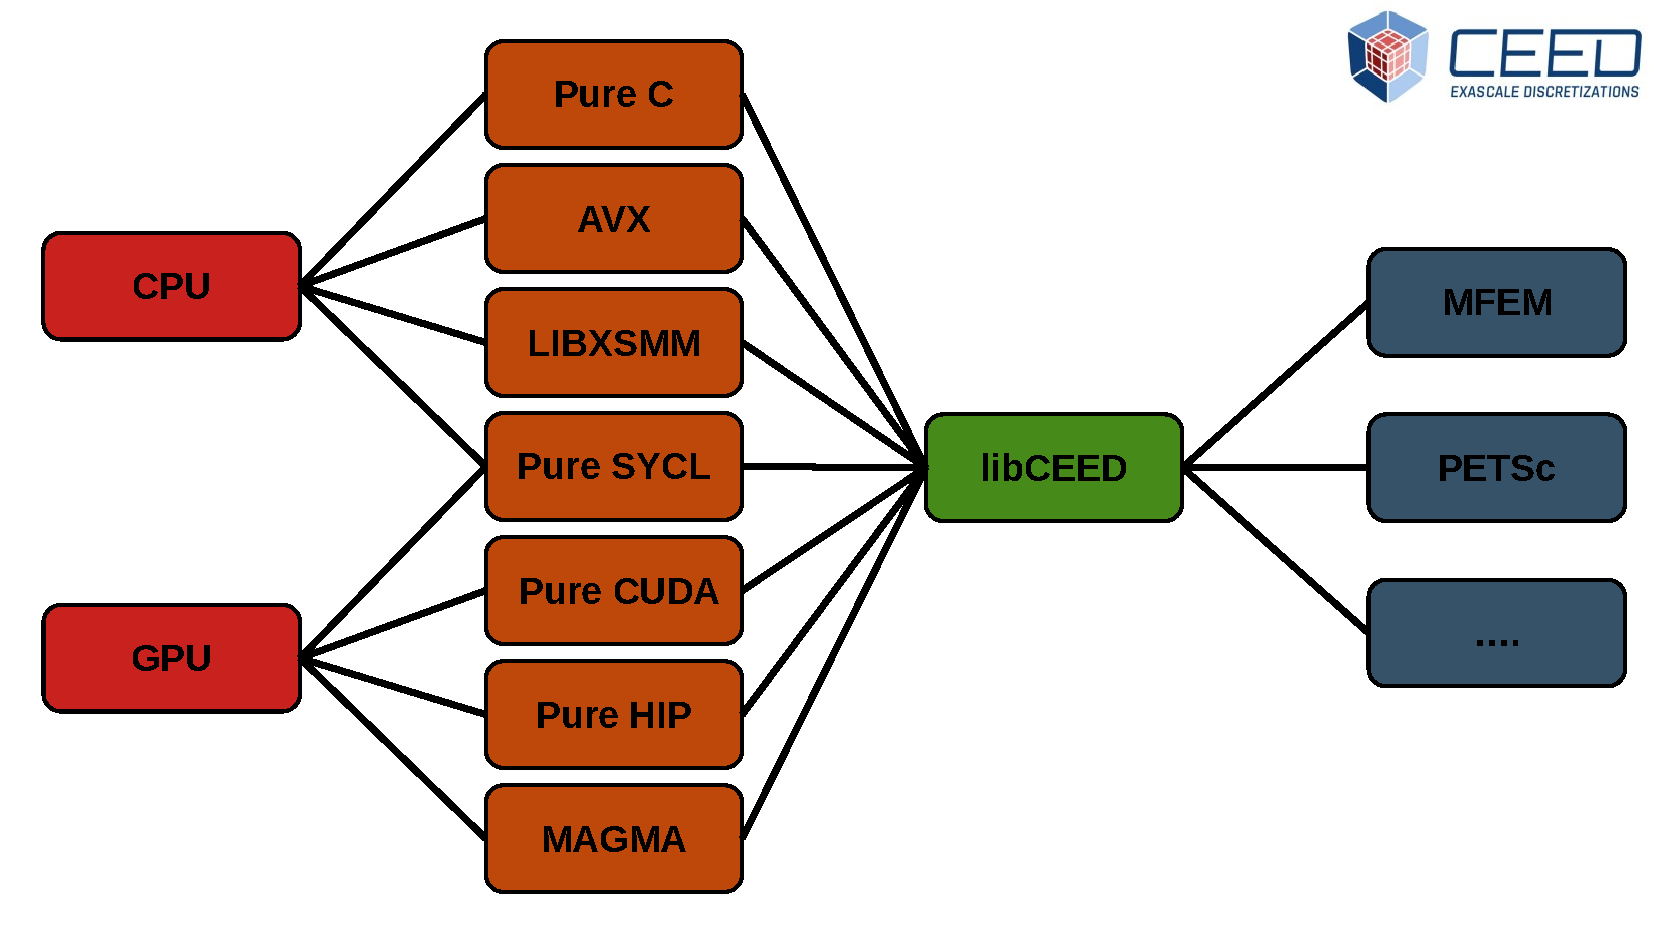
\includegraphics[height=5.5cm]{libCEEDBackends.pdf}

~\\

Performance portability with libCEED's matrix-free operators\\

\end{center}
\end{frame}

%------------------------------------------------

\begin{frame}[fragile]
\begin{center}
\frametitle{Extensible Solvers from PETSc}

\begin{columns}
  \begin{column}{.25\textwidth}
    ~\\
    \lstinline{CeedEvaluator}\\
    \vspace{1.75cm}
    \lstinline{MatCeed}\\
    \vspace{0.75cm}
    \lstinline{CeedVector}\\
  \end{column}
  \begin{column}{.75\textwidth}
    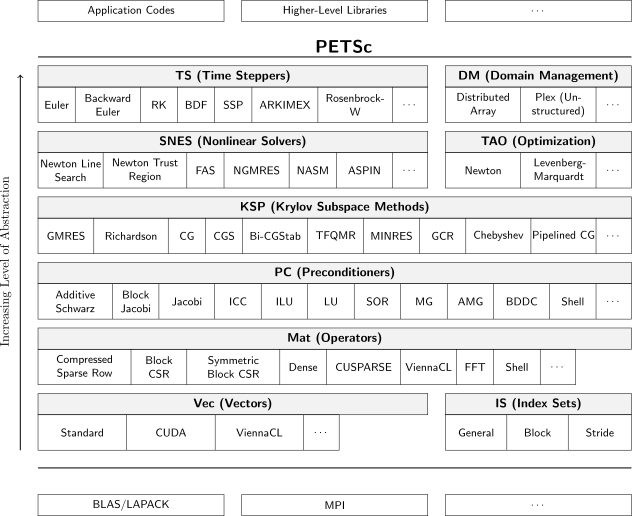
\includegraphics[height=6.0cm]{PETScAPI.png}
  \end{column}
\end{columns}

~\\

Need to wrap libCEED operators to work with PETSc objects\\

\end{center}
\end{frame}

%------------------------------------------------
\section{CeedEvaluator}
%------------------------------------------------

\begin{frame}[fragile]
\begin{center}
\frametitle{CeedEvaluator}

\lstinline{CeedEvaluator} wraps a non-linear \lstinline{CeedOperator}

{\tiny
\begin{lstlisting}[style=boxedC]
CeedEvaluatorCreate(DM dm_x, DM dm_y, CeedOperator op, CeedEvaluator *evaluator);
CeedEvaluatorUpdateTimeAndBoundaryValues(CeedEvaluator evaluator, PetscReal time);

// Different Apply* variants
CeedEvaluatorApplyGlobalToGlobal(CeedEvaluator evaluator, Vec X, Vec Y);
CeedEvaluatorApplyAddGlobalToGlobal(CeedEvaluator evaluator, Vec X, Vec Y);
CeedEvaluatorApplyVelocityGlobalToGlobal(CeedEvaluator evaluator, Vec X, Vec X_dot, Vec Y);
CeedEvaluatorApplyGlobalToLocal(CeedEvaluator evaluator, Vec X, Vec Y_loc);
CeedEvaluatorApplyLocalToLocal(CeedEvaluator evaluator, Vec X_loc, Vec Y_loc);
\end{lstlisting}
}

\lstinline{CeedBoundaryEvaluator} provides essential BCs via \lstinline{CeedOperator}

{\tiny
\begin{lstlisting}[style=boxedC]
CeedBoundaryEvaluatorCreate(MPI_Comm comm, CeedOperator op_dirichlet, CeedBoundaryEvaluator *evaluator);

// Override DMPlex BC computation
DMPlexSetCeedBoundaryEvaluator(DM dm, CeedBoundaryEvaluator evaluator);
\end{lstlisting}
}

\end{center}
\end{frame}

%------------------------------------------------

\begin{frame}[fragile]
\begin{center}
\frametitle{Material Models}

\lstinline{CeedEvaluator} supports residual and auxiliary comutations\\

~\\

\begin{itemize}

\item \lstinline{TSIFunction}\\

~\\

\item \lstinline{TSI2Function}\\

~\\

\item \lstinline{TSRHSFunction}\\

~\\

\item \lstinline{SNESFunction}\\

~\\

\item \lstinline{SNESObjective}\\

~\\

\item Diagnostic/output value computation

\end{itemize}

\end{center}
\end{frame}

%------------------------------------------------
\section{MatCEED}
%------------------------------------------------

\begin{frame}[fragile]
\begin{center}
\frametitle{MatCEED}

\lstinline{MatCEED} wraps a linear \lstinline{CeedOperator}

{\tiny
\begin{lstlisting}[style=boxedC]
MatCeedCreate(DM dm_x, DM dm_y, CeedOperator op_mult, CeedOperator op_mult_transpose, Mat *mat);
MatCeedSetTime(Mat mat, PetscReal time);

// COO assembly support
MatCeedCreateMatCOO(Mat mat_ceed, Mat *mat_coo);
MatCeedSetPreallocationCOO(Mat mat_ceed, Mat mat_coo);
MatCeedAssembleCOO(Mat mat_ceed, Mat mat_coo);

// Private - Core functionality
MatMult_Ceed(Mat A, Vec X, Vec Y)
MatMultTranspose_Ceed(Mat A, Vec Y, Vec X)

// Private - PC support
MatGetDiagonal_Ceed(Mat A, Vec D);
MatGetDiagonalBlock_Ceed(Mat mat_ceed, Mat *mat_block);
MatInvertBlockDiagonal_Ceed(Mat mat_ceed, const PetscScalar **values);
MatInvertVariableBlockDiagonal_Ceed(Mat mat_ceed, PetscInt num_blocks, const PetscInt *block_sizes, PetscScalar *values);

\end{lstlisting}
}

\end{center}
\end{frame}

%------------------------------------------------

\begin{frame}
\begin{center}
\frametitle{Native PC Support}

\begin{itemize}

\item \lstinline{PCNone} - :)\\

~\\

\item \lstinline{PCJacobi} - matrix free diagonal assembly\\

~\\

\item \lstinline{PCPBJacobi} - matrix free block diagonal assembly\\

~\\

\item \lstinline{PCVPBJacobi} - matrix free variable block diagonal assembly\\

~\\

\item COO assembly into AIJ for all other PCs

\end{itemize}

\end{center}
\end{frame}

%------------------------------------------------

\begin{frame}
\begin{center}
\frametitle{PCpMG}

\begin{tikzpicture}
\node[shape=circle,draw=black] (A) at (0,0) {$p_2$};
\node[shape=circle] (Al) at (-1.2,0) {Smooth};
\node[shape=circle,draw=black] (B) at (2,-2) {$p_1$};
\node[shape=circle] (Bl) at (0.8,-2) {Smooth};
\node[shape=circle,draw=black] (C) at (4,-4) {$p_0$};
\node[shape=circle] (Cl) at (4,-5) {Coarse Solve};
\node[shape=circle,draw=black] (D) at (6,-2) {$p_1$};
\node[shape=circle] (Dl) at (7.2,-2) {Smooth};
\node[shape=circle,draw=black] (E) at (8,0) {$p_2$};
\node[shape=circle] (El) at (9.2,0) {Smooth};
\path[->] (A) edge node[left=10, pos=.6] {Restriction} (B);
\path[->] (B) edge node[left=10, pos=.6] {Restriction} (C);
\path[->] (C) edge node[right=10, pos=.4] {Interpolation} (D);
\path[->] (D) edge node[right=10, pos=.4] {Interpolation} (E);
\end{tikzpicture}

MatCEED directly supports all operations except GAMG coarse solve

\end{center}
\end{frame}

%------------------------------------------------
\section{MPM Support}
%------------------------------------------------

\begin{frame}
\begin{center}
\frametitle{What is MPM?}

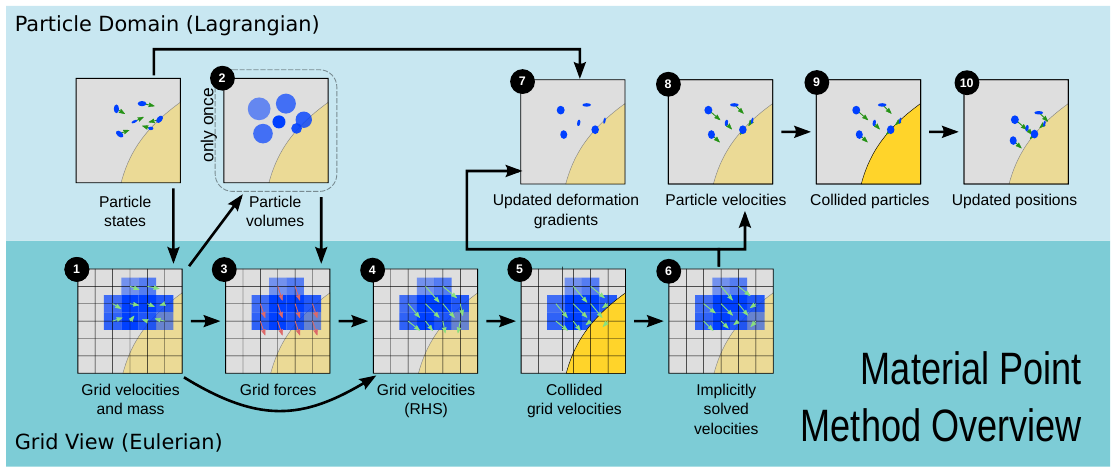
\includegraphics[height=5cm]{MPMOverview.png}\\

~\\

\begin{itemize}

\item Continuum based particle method with background mesh for gradients\\

\item Extension of FLIP (which is an extension of PIC)\\

\item Used in rendering for the movie \emph{Frozen}\\

\end{itemize}

\end{center}
\end{frame}

%------------------------------------------------

\begin{frame}
\begin{center}
\frametitle{What does MPM have to do with FEM?}

\begin{itemize}

\item Problem on background mesh changes when material points move\\

~\\

\item Natural fit for matrix-free representation\\

~\\

\item Similar reasoning to use matrix-free for adaptive methods\\

~\\

\item Ratel FEM infrastructure provides fast background mesh solves\\

\end{itemize}

\end{center}
\end{frame}

%------------------------------------------------

\begin{frame}
\begin{center}
\frametitle{libCEED Basis Evaluation AtPoints}

\begin{center}
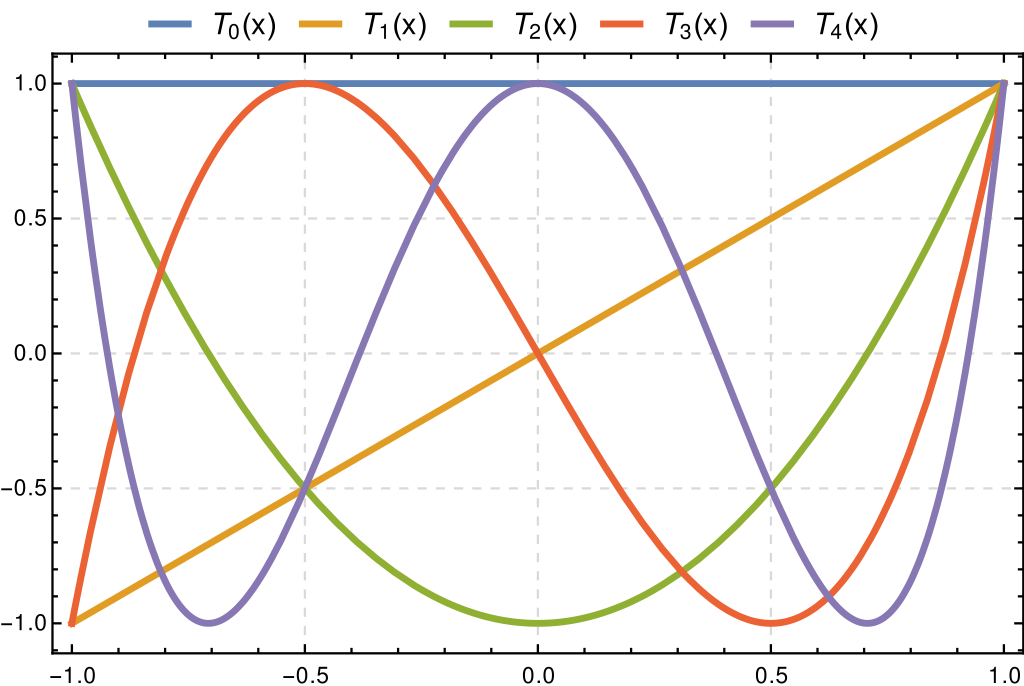
\includegraphics[height=4cm]{ChebyshevPolynomials.png}
\end{center}

\begin{itemize}

\item Interpolate from primal to dual (quadrature) space\\

\item Fit Chebyshev polynomials to values at quadrature points\\

\item Evaluate Chebyshev polynomials at reference coords of material points\\

\item Transpose the order for projection to mesh from material points\\

\end{itemize}

\end{center}
\end{frame}

%------------------------------------------------

\begin{frame}
\begin{center}
\frametitle{DMSwarm for Material Points}

\begin{center}
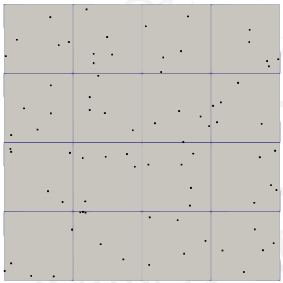
\includegraphics[height=4cm]{DMSwarmOverview.png}
\end{center}

\begin{itemize}

\item DMSwarm manages material points\\

~\\

\item DMPlex manages cells (elements)\\

~\\

\item API for cell reference coordinates of points\\

\end{itemize}

\end{center}
\end{frame}

%------------------------------------------------

\begin{frame}
\begin{center}
\frametitle{Current MPM Work}

\begin{itemize}

\item CeedOperator support AtPoints on CPU\\

~\\

\item GPU support - ElemRestriction complete, Basis in progress\\

~\\

\item Ratel implements MPM for CEED BPs, elasticity in progress (soon)\\

\end{itemize}

\end{center}
\end{frame}

%------------------------------------------------
\section{Future Work}
%------------------------------------------------

\begin{frame}
\begin{center}
\frametitle{Future Work}

\begin{itemize}

\item CeedEvaluator\\

\begin{itemize}

\item Further testing in Ratel/HONEE desirable

\item Need API for arbitrary number of input/output vectors

\end{itemize}

~\\

\item MatCEED\\

\begin{itemize}

\item Ready for initial upstreaming

\item Wrap inner AIJ for other PCs (GAMG!)

\end{itemize}

~\\

\item Develop QFunction specification (resolution independent)\\

~\\

\item We invite contributors and friendly users\\

\end{itemize}

\end{center}
\end{frame}

%------------------------------------------------

\begin{frame}
\frametitle{Questions?}

\begin{center}
\includegraphics[height=2.75cm]{libCEEDlogo.png}
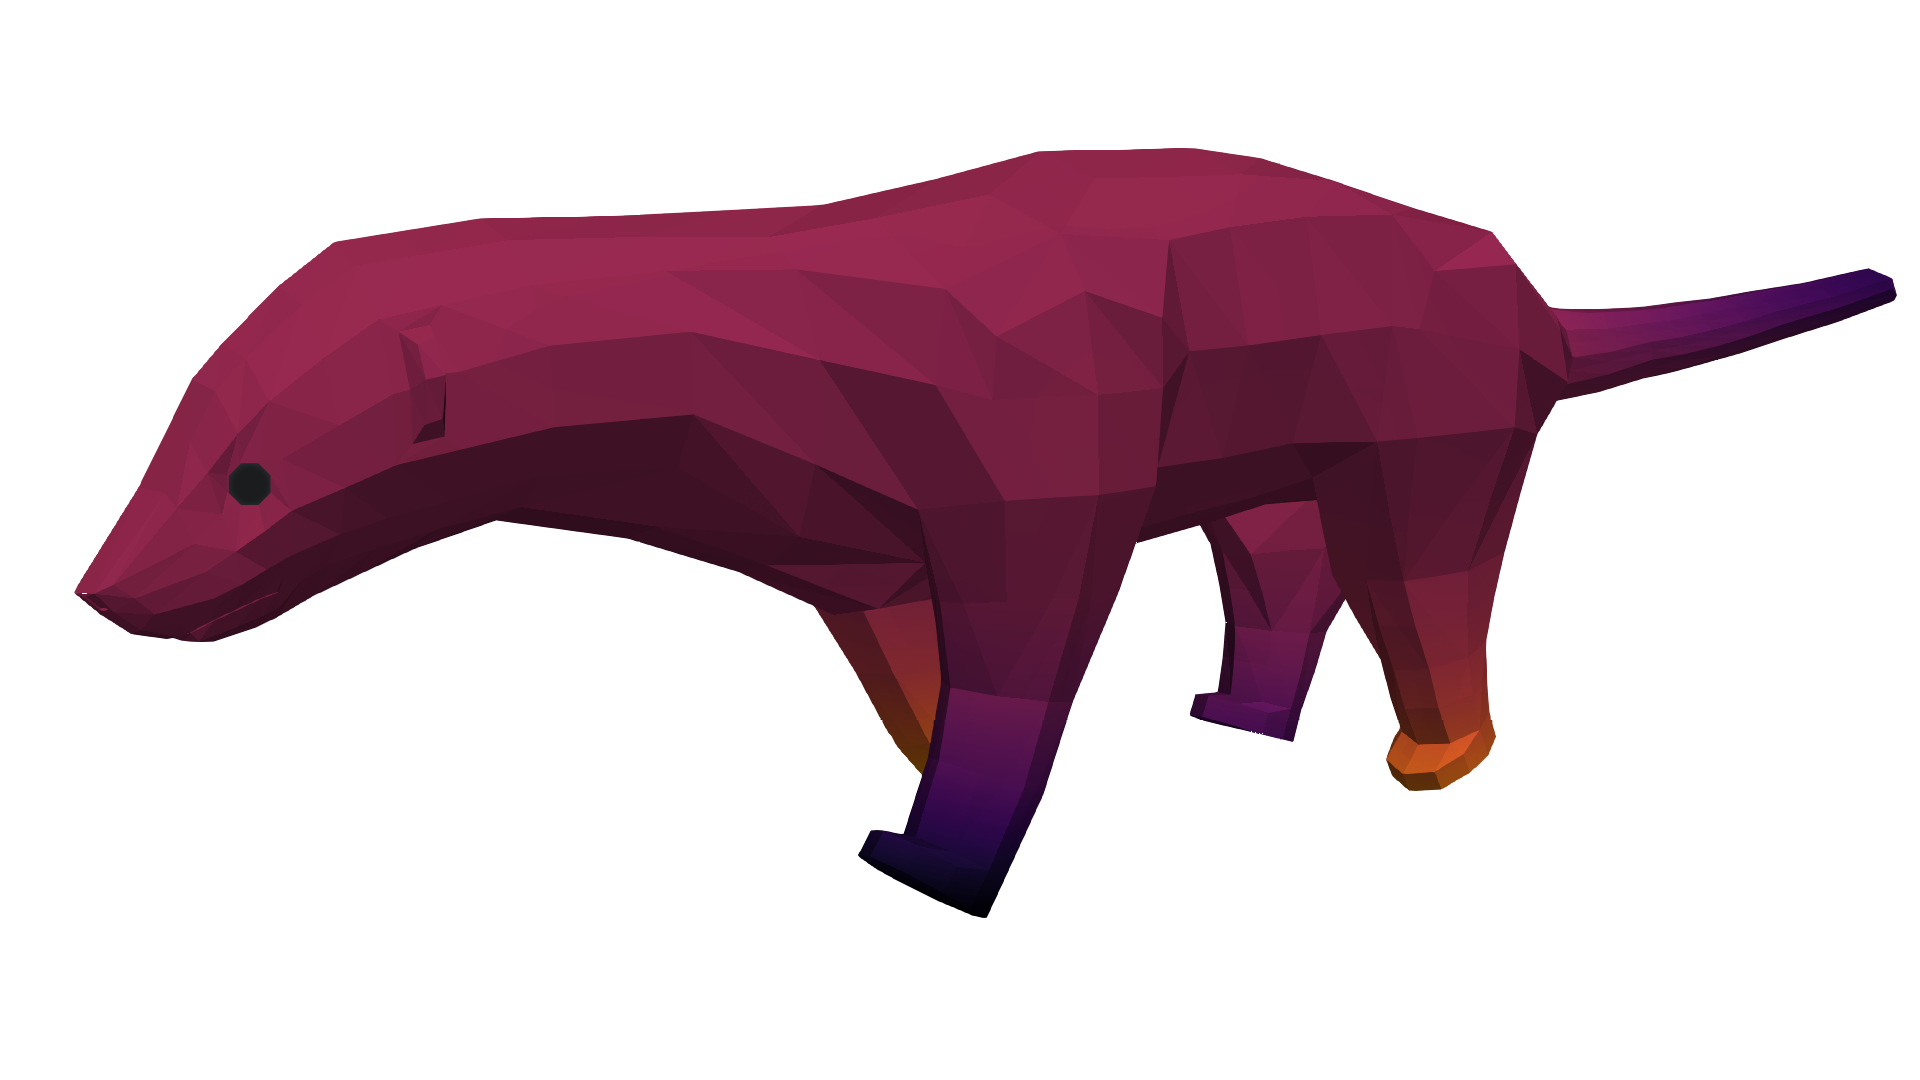
\includegraphics[height=2.75cm]{Ratellogo.png}
\end{center}

{\flushleft

libCEED Repo: https://github.com/CEED/libCEED\\
Ratel Repo: https://gitlab.com/micromorph/ratel\\

~\\

Grant: Predictive Science Academic Alliance Program (DE-NA0003962)\\

}

\begin{center}

\includegraphics[height=0.8cm]{psaap-center-logos}
\end{center}

\end{frame}

%-------------------------------------------------------------------------------

\end{document}

%-------------------------------------------------------------------------------
